\documentclass{NSF}

\usepackage{xspace}
\newcommand{\BfPara}[1]{{\noindent\textbf{#1.}}\xspace}
\newcommand{\etal}{{\em et al.}\xspace}
\newcommand{\etc}{{etc.}\xspace}
\newcommand{\ie}{{\em i.e.}\xspace}
\newcommand{\eg}{{\em e.g.,}\xspace}
\usepackage{marvosym}

% Let us define our framework name HERE!
\newcommand{\ours}{RFlow$^+$}
\newcommand{\ourIs}{InstaMeasure}
\newcommand{\ourFR}{FlowRegulator}
\begin{document}


% B. Project Summary
\title{Research Statement}\\
%\name{Rhongho Jang}
\\\rule{\textwidth}{1.5pt}\vspace{3mm}
%\Mobilefone{ +1 (407) 840 8881\ \ \ \ \       }
%\Mobilefone{ +82 (10) 2052 7777}\\
%{\textbf{Email}: r.h.jang@knights.ucf.edu}
%\vspace{-8mm}

My research interests are focused on the security of blockchains and distributed systems. My Ph.D., work is dedicated to a systematic exploration of the blockchain attack surface actuated by the cryptographic constructs of the blockchain data structure, the peer-to-peer network formed by the blockchain nodes, and the application-specific deployment of blockchain systems in cryptocurrencies, smart contracts, and audit logs. My work in the blockchain security has led to the discovery of (1) DDoS attacks on blockchain memory pools, (2) partitioning attacks on the Bitcoin network, (3) asynchrony in the real-world blockchain systems, and (4) illicit mining through web browsers through cryptojacking. Concurrently, I have developed countermeasures for these attacks by proposing refinements to the existing blockchain consensus protocols, designing optimal network setups that facilitate secure information exchange, and constructing application-layer remedies. All these works have been consolidated in the first systematic survey on the blockchain attack surface published in the prestigious IEEE Communication Surveys and Tutorials 2020. 


Alongside the attack surface analysis, I pursued two other thrusts in blockchain systems. First, I have used cryptocurrency network artifacts to develop machine learning models for price prediction. My work on Bitcoin and Ethereum price prediction won the best paper award at IEEE Systems Journal 2019. Second, I have worked on instrumenting the requirements for legacy systems where blockchain primitives can be usefully applied to achieve security and provenance. In that space, I have used blockchains in the audit applications to (1) harden their security by distributed control among application instances, and (2) ensure provenance by logging system events in an append-only ledger. My work on secure and transparent blockchain-based audit logs won the best paper award in DLoT 2018.   


In terms of novelty and impact, the most notable projects in my research are related to the partitioning attacks which I have incorporated in my dissertation. In the following, I briefly discuss those works along with my future research plans. 


\section{Ph.D. Dissertation}

\BfPara{Partitioning Attacks} In the first thrust, I set forth the concept of spatial, temporal, spatio-temporal, and logical partitioning attacks on the Bitcoin network. In the spatial partitioning attack, I reported the increasing centralization of Bitcoin nodes across the Autonomous Systems (ASes) which put them at a high risk of routing attacks. In the temporal partitioning attacks, I observed weak network synchronization over the blockchain ledger, indicated by an unexpectedly high diversity in the blockchain view of each Bitcoin node. In the spatio-temporal partitioning attacks, I located the intersection between the aforementioned partitioning types to amortize the attack cost and amplify the attack implication on the network. Finally, in the logical partitioning attack, I studied the software vulnerability across dominant the Bitcoin Core deployments that posed serious risks to the Bitcoin users. For each attack type, I also proposed countermeasures one of which was an independent work ({\em RouteChain}) that aimed at straightening the Border Gateway Protocol (BGP). The work on partitioning attacks appeared in the notable distributed systems conference (ICDCS 2019), and {\em RouteChain} appeared in (ICBC 2019). The work contributed in causing awareness in the research and development community. Recently, Bitcoin Core has incorporated a technique called {\em asmap} that creates AS-level diversity among Bitcoin nodes. 

\BfPara{HashSplit Attack} In the second thrust, I examined the effect of Bitcoin communication model on the blockchain {\em safety}. First, I constructed the Bitcoin ideal-functionality that preserves the common-prefix and chain-quality properties in under {\em lock-step} synchronous and {\em non lock-step} synchronous communication model. Next, I set up a large measurement apparatus to detect mining and non-mining nodes and monitor the information flow among them Bitcoin. The results revealed a high disparity in the ideal functionality and the real-world deployment, showing that the Bitcoin network is actually asynchronous which can be exploited to violate the blockchain {\em safety} properties and amortize the cost of 51\% attack. The work also draws attention to the gap between the theory and practice since the applied nature of network asynchrony is not discussed in the research and development community. To bridge the gap, I modified Bitcoin Core to closely emulate the {\em lock-step} synchronous network and resist asycnhrony. The work is currently under review in S\&P 2021. 


\BfPara{Root Cause Analysis} The third thrust performs the root-cause analysis for weak network synchronization which is antecedent to temporal partitioning attacks. In the prior two thrusts, we presumed that weak network synchronization is due to block propagation delay caused by network size and communication overhead. Our assumption was inspired from prior notable works that established a relationship between network size and blockchain synchronization. However, recent data from 2020 reveals that the relationship does not hold in practice. Since 2019, the Bitcoin network size has reduced by 8\% and unexpectedly, the network synchronization has also reduced by 15\%. This observation mandates that we 


% My research interests are focused on network monitoring system design, anomaly detection, and traffic engineering. During my Ph.D. study, I worked on several research projects, such as rogue access point detection, website fingerprinting, traffic measurement algorithms, and network monitoring systems. Among these projects, my core research topics are traffic measurement algorithms and monitoring systems design. My works can be divided into three thrusts. In the first thrust, I designed a scalable per-flow measurement algorithm based on compact data structures (i.e., sketches), towards performing line-speed traffic measurements with small memory space and computational overhead (work accepted by INFOCOM 2020). In the second thrust, I integrated my sketch into the SDN framework. As a prototype, I proposed a two-level network monitoring mechanism and then deployed it in an off-the-shelf wireless router (published in INFOCOM 2017). Further, I achieved online (Layer 4) per-flow monitoring using Atom CPU at a campus gateway (published in ICDCS 2019). The last thrust is sketch measurement under the Tofino environment by implementing all well-known sketches in the Tofino and evaluating their performance. Particularly, my core research plan is to deliver new insights for those who want to design sketch-based monitoring systems by answering the following (1) how many hash calculations are acceptable? (note that sketches are usually hashing-heavy), (2) can ASIC be tolerant when sending data heavily to the user-space? (the other feature of the sketch), and (3) how to monitor fine-grained (L4) flows using only the SRAM and DRAM instead of the expensive and small TCAM? Eventually, my goal is to design a cost-efficient L4-per-flow monitoring system in Tofino, then using fine-grained flow statistics to support decisions in anomaly detection and traffic engineering. 
% In the following, I would like to highlight my interests by sampling my research using two dissertation works (at UCF and INHA University) and discuss my future research plan.

\section{Ph.D. Dissertation 1 at the University of Central Florida}
In the zettabyte era, per-flow measurement becomes more challenging for the data center owing to the increase of both traffic volumes and the number of flows. Also, the swiftness of the detection of anomalies (\eg congestion, link failure, and DDoS attack) becomes paramount. 

\BfPara{Scaling Up Per-flow Measurement using DRAM} For fast and accurate traffic measurement, managing an accurate working set of active flows (WSAF) from massive volumes of packet influxes at line rates is a key challenge. WSAF is usually located in high-speed but expensive memory, such as TCAM or SRAM, and thus the number of entries to be stored is quite limited.
To cope with the scalability issue of WSAF, in the first phase of this dissertation, we propose to use In-DRAM WSAF with scales and put a compact data structure (\ourFR{}) in front of WSAF to compensate for DRAM's slow access time by substantially reducing massive influxes to WSAF without compromising measurement accuracy. 
To verify its practicability, we further build a per-flow measurement system, called \ourIs{}, on an off-the-shelf Atom (lightweight) processor board.
We evaluate our proposed system by a large scale real-world experiment (connected to monitoring port of our campus main gateway router for 113 hours, and capturing 122.3 million flows). 

\BfPara{Scaling Up Per-flow Measurement Using Sampling} In the second piece of this dissertation, we aimed to design a novel sampling scheme to deal with the poor trade-off provided by random sampling. 
Starting with a simple idea that "independent per-flow packet sampling provides the most accurate estimation of each flow," 
we introduced a new concept of per-flow systematic sampling, 
to provide the same sampling rate across all flows. 
Besides, we realized the design of a concrete sampling method called SketchFlow, which approximates the idea of the per-flow systematic sampling using a sketch saturation event.

\BfPara{System Integration} For the last part of this research project, and system-wide, we proposed an SDN-based WLAN monitoring and management framework called \ours{} to address WiFi service dissatisfaction caused by the limited view (lack of scalability) of network traffic monitoring and absence of intelligent and timely network treatments.
Existing solutions (e.g., OpenFlow and sFlow) have a limited view, no generic flow description, and a poor trade-off between measurement accuracy and network overhead depending on the selection of the sampling rate.
To resolve these issues, we devise a two-level counting mechanism, namely a distributed local counter (on-site and real-time) and central collector (a summation of local counters). With this, we proposed a highly scalable monitoring and management framework to handle immediate actions based on short-term (\eg 50 ms) monitoring and eventual actions based on long-term (\eg one month) monitoring. 
The former uses the local view of each access point (AP), and the latter uses the global view of the collector. 
%Experimental results verify that \ourIs{} can achieve high accuracy (less than 5\% standard error for short-term and less than 1\% for long-term) and fast detection of flows of interest (within 23 ms) with manageable network overhead.
%We prove the practicality of \ourIs{} by showing the effectiveness of a MAC flooding attacker/a super-spreader quarantine in a real-world testbed.



\section{Ph.D. Dissertation 2 At INHA University}
In this research project, we introduce a powerful hardware-based rogue access point (PrAP) that acts as a man-in-the-middle attacker by relaying back and forth traffic between a legitimate AP and wireless stations. Our PrAP is physically interconnected using two dedicated wireless routers, and can send traffic rapidly between and a legitimate AP and victim stations. Through experiments, we show that the state-of-the-art time-based rogue AP (rAP) detection scheme cannot detect our PrAP, although it is effective against software-based rogue AP. In explaining that, we reveal new insight into the fundamentals of time-based detectors for software-based rogue APs and their operations: these techniques are only capable of detecting software-based rogue APs due to the speed of wireless AP bridging. To address the threat of the PrAPs, we propose a new detection tool for network administrators, a PrAP-Detector based on intentional channel interference. Our PrAP-Detector is highly accurate in various traffic scenarios: idle and heavy traffic.
Further, we prototype our PrAP-Detector using a high-end desktop and a smartphone. We demonstrate a close to 100\% detection rate, compared to a 60\% detection rate of the state-of-the-art scheme. We show that our PrAP-Detector is fast (5-10 seconds detection time), doesn't require prior knowledge, and can be deployed in the wild by conducting real-world experiments at ten coffee shops.

\section{Future Research Plan}
We are inching closer to the zettabyte era with the ever-increasing volumes of traffic on the Internet. 
%In 2016, 90\% of the world's data had been created in the previous two years. (Source: IBM). In 2019, Twitter users sent more than 500,000 tweets every minute. (Source: Domo). 
By 2023, there will be around 100 zettabytes of data (Source: EMC). 
%This is because IT becomes one of the most important parts of human life, and demands on quality are increasing as well. For instance, the demand for ultra-high resolution images and high-definition video is one of the factors of rapidly increasing data volumes. 
The increasing data volumes not only accelerated the development of processing, storage, and I/O devices but also the network infrastructure. As of now, the per-port speed of network devices reached 100 Gbps, and high-end switches are capable of processing more than 25.6 Tbps of network traffic. 

As one of the key functionality of such devices, network traffic measurement is crucial in many fields, such as billing, load balancing, anomaly detection, intrusion detection, and network failure detection. However, network traffic measurement is still at an early stage and facing various challenges. 
%The main reason is the constrained processing and memory resources of the switch. 
In practice, traffic measurement relies on either sampling or advanced devices. To ensure online processing, Cisco's NetFlow maintains flow information in TCAM and their statistics in SRAM. However, the number of entries in the table cannot be large because those memory chips are expensive. Instead, sFlow sends the collected packet headers (i.e., samples) periodically to a collecting server over the network to minimize the overhead in the data-plane. However, it presents a Control Loop 
%(i.e., measurement delegation caused detection/control delay) 
between the server and switch, which leads to inaccurate analysis and delayed detection/response. To this end, any measurement system falls into either one of these two models. 
%Besides, with the advancement of Internet services, more traffic will be processed at higher speed, which means that traffic measurement and corresponding detection (faults, attacks) within the switch are not only essential but also should be accurate. 
A large body of research works is proposed to address these issues, although most such work is impractical due to various limitations. Moreover, none of such work is commercialized.

For per-flow measurement, sketch-based techniques have been greatly enhanced over several decades. To date, sketch-based techniques are still one of the most active research topics with results published in major conferences (i.e., USENIX NSDI, ACM SIGCOMM, IEEE INFOCOM, IEEE ICDCS \etc). Unlike their counterparts (\eg Netflow, sFlow, jFlow, \etc), sketch-based counting algorithms require a small amount of memory to measure a large volume of traffic.% in real-time. 
%To decrease memory usage, most works have used statistically shared counters, matrices, and Bloom filters as statistical noise from each estimation can be removed at the time of estimation (or decoding). To enhance estimation accuracy, maximum likelihood estimation is usually adopted, thereby introducing a substantial amount of additional computations. 
Even though the sketch-based techniques are promising in traffic measurement, they are faced with two major problems. First, most of the sketch-based decoding algorithms involve hundreds of hash calculations (i.e., computationally hard) and memory accesses from statistically mixed random blocks to obtain meaningful statistics (e.g., heavy hitters, DDoS attack, flow size distribution and entropy, etc.). Second, sketches are quickly saturated. Sketch maximizes the efficiency and utilization of memory space but cannot last for a long time. Due to the limited memory space, a large volume of traffic eventually saturates sketches, forcing the saturated sketches to be sent to a remote collector, which leads sketches to fall into a Send-and-Decode model.

The Send-and-Decode model is commonly accepted in practice but inherently incurs huge network bandwidth overhead and network delay. Notably, for switches that are wildly used in data center servers, remote decoding undoubtedly increases the network congestion, which degrades the user experience. Thus, in-data-plane decoding and processing are highly necessary for instant measurement and further timely detection.

\subsection{High-level System Designs and Goals}
\begin{figure}[b]
  \centering
  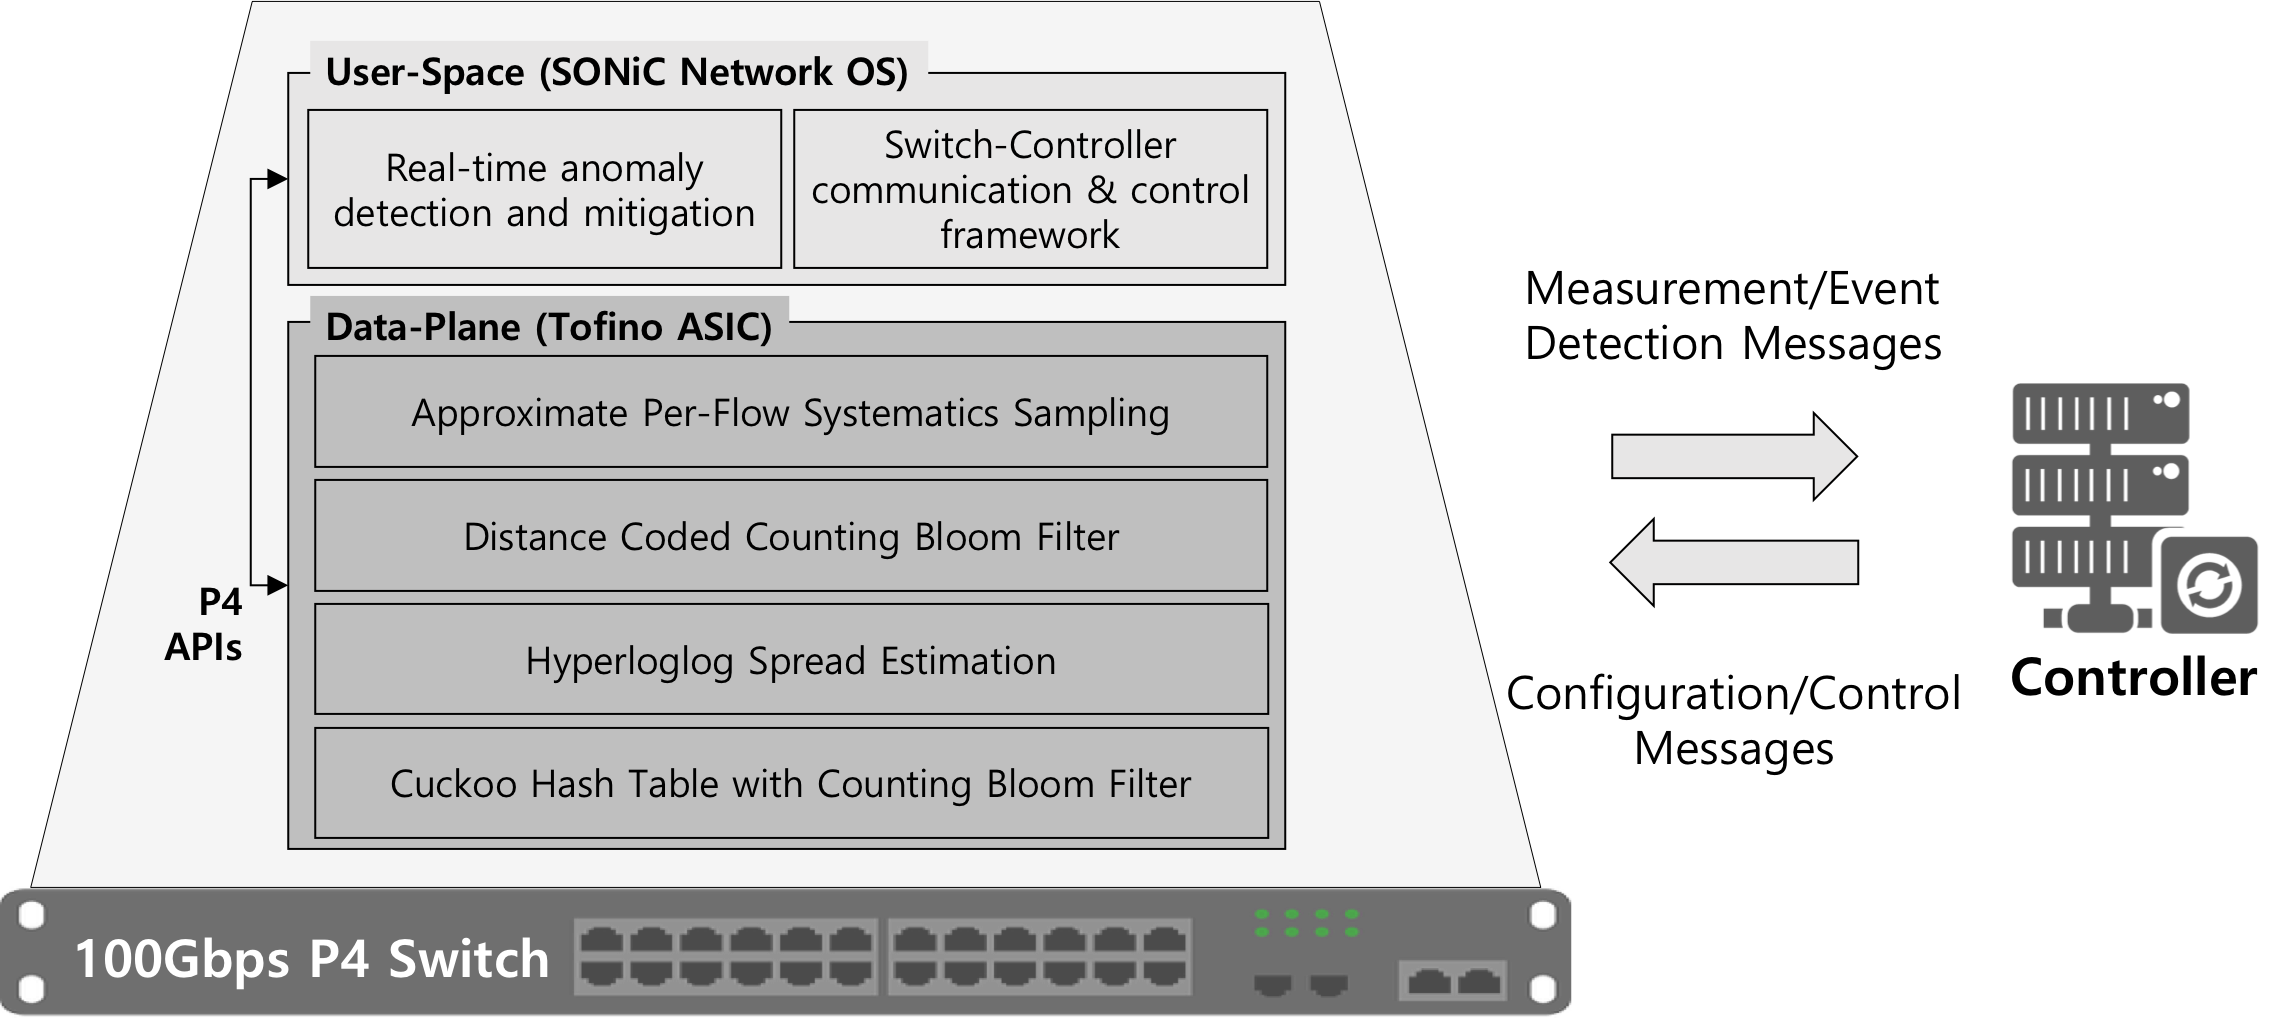
\includegraphics[width=0.8\textwidth]{fig/Vision.png} 
  \caption{The high-level designs and goals of future research}
\end{figure}

The primary focus of my further research is to enable in-data-plane scalable traffic measurement and timely detection. Figure 1 shows the vision of my further research. The eventual goal of this research is not only proposing in-data-plane traffic measurement data structures and algorithms but also building a complete network device communication system that supports a network-wide measurement to deal with more comprehensive problems, such as network traffics engineering and anomaly detection. The algorithms are expected to be implemented in the commercial switch using data-plane programmable features of Intel's Barefoot Tofino ASIC. Moreover, the system-wise designs will strictly follow the state-of-the-art standards and contributed to the commercial/opensource switch system projects. 



\BfPara{Thrust 1: Sketch-based Flow Sampling/Counting Technology}
At the core of our system, we proposed a highly scalable and efficient in-data-plane per-flow sampling/counting algorithm to enable fine-grained (5-tuple) flow measurements under a high-speed and high-volume environment. Different from other sketches, our sketch is characterized as a low-cost data structure that can fit into a memory-constrained switch device and guarantees online performance. As known, sampling is a powerful tool to reduce the processing overhead in various systems. However, the wildly used Simple Random Sampling (SRS) approach samples packets over an aggregated data flow (defined by switch port or VLAN) and provides pool accuracy for different fine-grained flows (defined by the 5-tuple). 
 %Figure 2 (right figure) shows the accuracy of our core algorithm, namely SketchFlow. For each flow, the fraction of the sampled packet number over the flow sizes almost equivalent to the sampling rate of 1/p. Moreover, the variance of SketchFlow is much smaller than the simple random sampling scheme (left figure).
We stress that the scalable fine-grained per-flow measurement is a missing function in most of the commercial switches, because of the constrained resources. The SRS approach was an alternative but is barely used in practice due to poor accuracy. Our sampling approaches will ensure the accuracy of 2nd-Order-statistic; even when the collected subpopulation is dreamily smaller than the full population data. With our core algorithms, we opened new potentials to achieving fine-grained traffic engineering and anomaly detection using real-time provided fine-grained per-flow statistics. 

% \begin{figure}
%   \centering
%   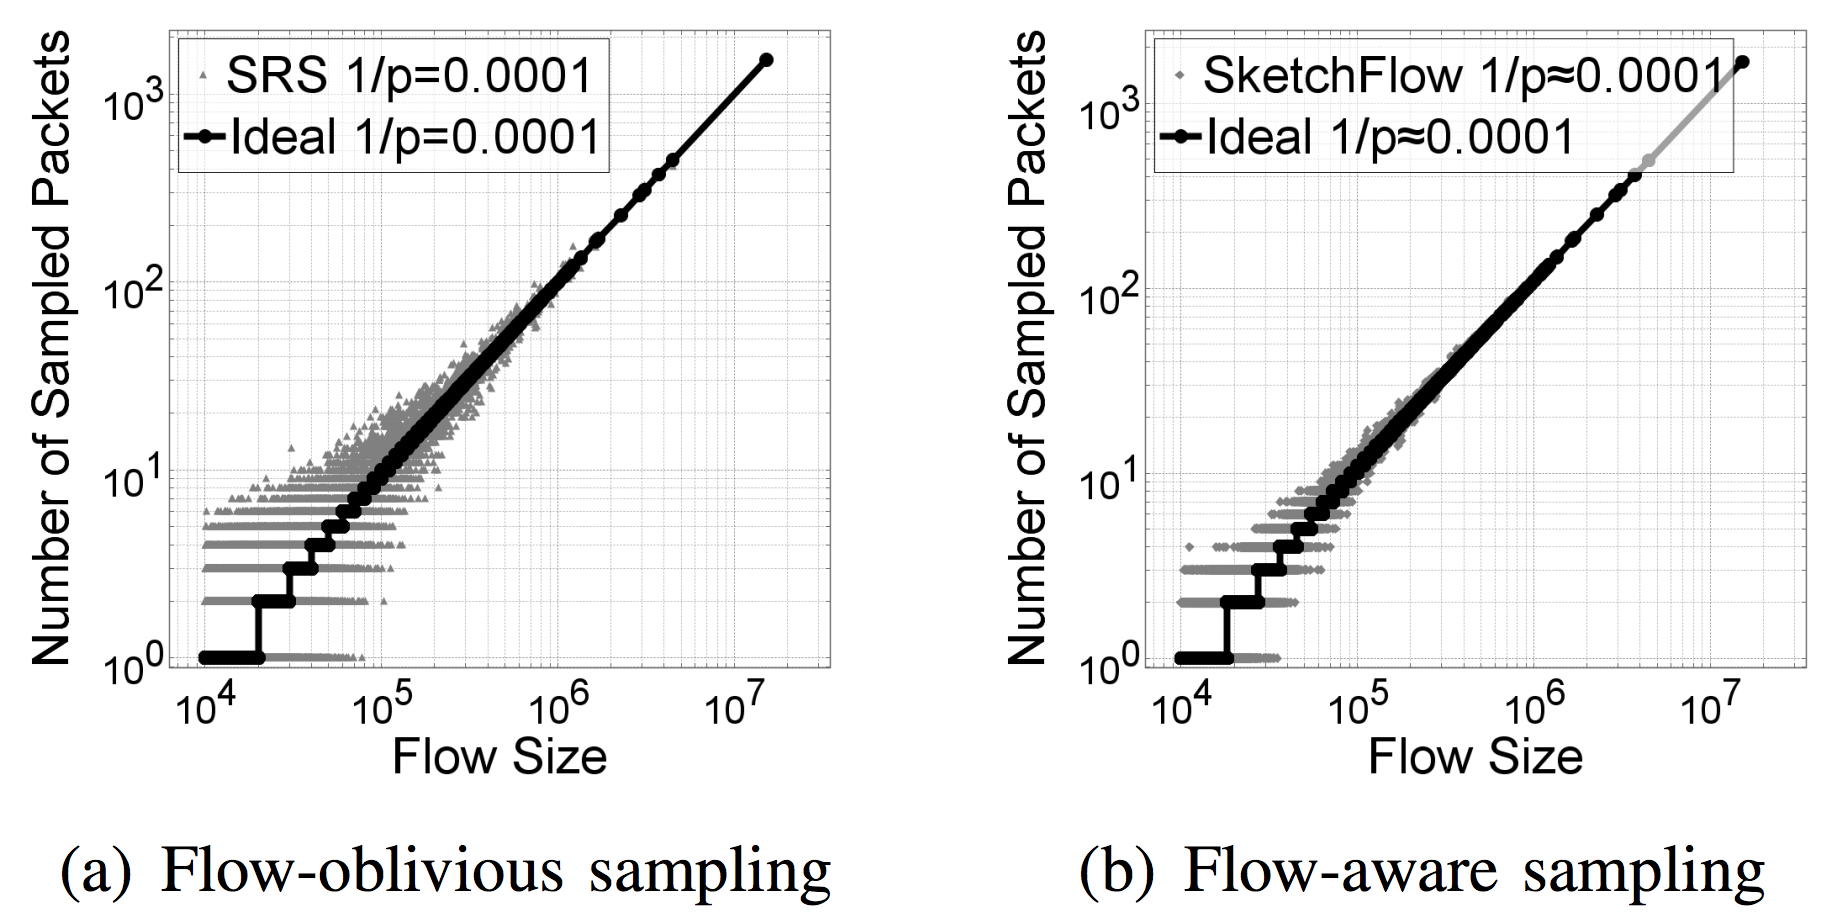
\includegraphics[width=0.8\textwidth]{fig/fig2.png} 
%   \caption{Simple Random Sapling (SRS) vs. Approximated Per-flow Sampling (SketchFlow) vs. Exact Per-flow Sampling (Ideal).}
% \end{figure}

\BfPara{Thrust 2: Per-flow Spectral Density Distribution Measurement Technology} 
In this thrust, we focus on the sketch saturation problem. As discussed above, sketches can maximize the efficiency of memory usage but eventually will be saturated by accumulated inflex information. One way to solve this problem is to recycle the memory space of inactive flows, which is very hard because the bit positions are not dedicated to individual flows. The other way is to mitigate the per-flow memory usage of the sketch. Instead of increasing bit position occupation to sketch the volume of flows, we use a computational distance to indicate the volume of flows, namely Distance-Coded Bloom Filter. In this way, we can minimize the memory space assigned for each flow to scale up the flow counting and retention capacities.

\BfPara{Thrust 3: Per-flow Spread Distribution Measurement Technology}
Spreader detection is essential in terms of anomaly detection, such as spammer detection, Distributed Denial-Of-Service (DDoS) attack. Although the estimation of spreader can be driven by spectral density distribution, however, it is impractical to be placed in data-plane because of the computational overhead of its operations (extensive memory read). Moreover, given that the most critical attacks (\eg DDoS attack) usually generate a high volume and high entropy traffic within a short time, the measurement and detection are highly required to be lightweight and can be performed in a timely manner. In this thrust, we mainly focus on designing an in-data-plane decodable spreader detector that can be deployed in commercial switches (data-plane programmable switch) to detect spreader-related anomalies in real-time. 

\BfPara{Thrust 4: Scalable Flow Record Hash Table} 
%Flow record table can be found in all commercial switches and routers, which are usually stored in TCAM  or SRAM for switching or routing purposes. 
%NetFlow uses TCAM to parallel match flow IDs and lookup the corresponding actions or updates the flow counting volumes in the SRAM.
%However, the number of entries in the table cannot be large because those types of memories are quite expensive. 
Flow record table is stored in fast-but-small TCAM or SRAM for switching purposes. 
For scalability, we can put the flow record table in DRAM instead of the expensive memory. 
%(i.e., an incentive to cost-effectiveness). However, there is a speed issue for the In-DRAM flow record table: a packet arrival rate is too fast to handle in the DRAM, owing to the DRAM's slow access speed 
Nevertheless, DRAM's slow access time
(roughly ten times slower than TCAM and SRAM) and the hash collision is shortcomings. One way to compensate for the slow DRAM is to use sampling techniques to mitigate the influx rate of the hash table, which has been shown is efficient in our previous work (InstaMeasure; IEEE ICDCS 2019). However, a hash collision of the flow table is another problem. 
To address this problem, we will design a sketch-guided cuckoo hash table that can drastically reduce the number of the access time of DRAM. The initial design of our new sketch is to use a counting bloom filter to indicate the horizontal location of the flow entry in the cuckoo hash table. Combining that with the vertical location information, we can access the flow record with minimum DRAM accesses. 
%As shown in Figure 3, the DRAM access time of our initially designed flow record table is stably near one over time, which can minimize the computational overhead caused by the hash collision. 
System-wise, we plan to fit the sketch into on-chip designed SRAM of data-plane (ASIC Switch) to reduce the flow entry locating the time and put the flow record table in the user-space DRAM. By doing so, we expect to achieve efficiency and scalability at the same time. 

%  \begin{figure}
%   \centering
%   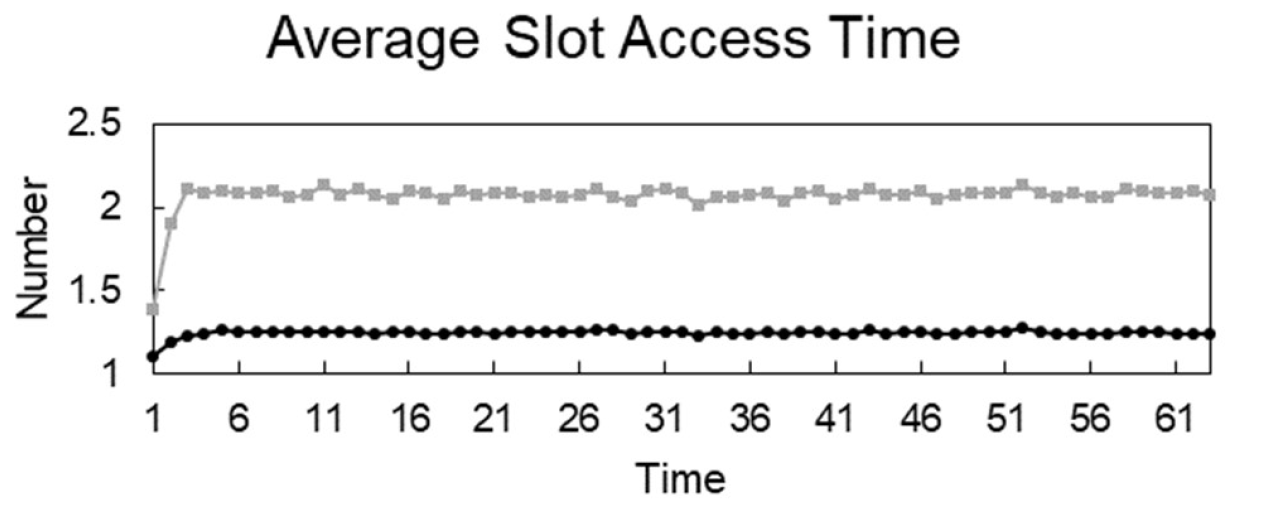
\includegraphics[width=0.8\textwidth]{fig/fig3.png} 
%   \caption{The average DRAM access time of our hash table. Gray rectangles show the average DRAM access time of the original cuckoo hash table, and the Black circles stand average DRAM access time of our initially designed flow record table.}
   
% \end{figure}
 

\BfPara{Thrust 5: Onsite Anomaly Detection and Mitigation}
Since the in-data-plane measurement is almost impossible using current technologies, traffic measurement is usually delegated by off-loading, sending sample packet headers, or accumulating temporally stored flow records to a remote server, leading to a Control Loop (delayed detection, mitigation, and control) between switches and controllers. In this thrust, we will focus on using a pre-defined rule sets to guide mitigation and control malicious flows in a local and timely manner (switch). By taking advantage of our proposed in-data-plane decodable data structures, the goal is to achieve an online detection of anomalies. For achieving more intelligent mitigation and control of networks, we expect to take advantage of machine learning techniques to dynamically predict and define the action sets.

\BfPara{Thrust 6: Controller-and-Switch Communication Framework Integration}
Our eventual goal is not only realizing the in-data-plane detection and mitigation but also achieving a network-wide defense and control. To do so, a centralized statistic collection server and control server are needed. The focus of this thrust is the use of fine-grained per-flow statistics from data-plane to achieve network-wide anomaly detection and information-driven precise traffic engineering. Previously proposed approaches are impractical to be integrated into an opensource switch system and software (\eg SONiC, Open Network Linux \etc). Instead of proposing a new framework from scratch, we will make efforts to embed our proposed data structures and algorithms into the opensource systems, and strictly following the state-of-the-art standards. For those designs that have not been standardized, we will actively make contributions to the future standard. 

\section{Potential of Attracting Funding}\vspace{-1mm}
The core of my work and associated thrusts are quite timely, and will be of interest to both academia and the industry, and have the potential of attracting funding from the industry, local state sponsors, as well as national funding agencies (\eg NSF, NRF). In terms of academia, the recent network specialized major conference ACM CoNEXT (The 15th International Conference on emerging Networking EXperiments and Technologies, held between Dec 9 and Dec 12, 2019, and co-organized by my advisor) had a full session on the data-plane programmable networks. Moreover, top-tier conferences (ACM SIGCOMM and USENIX NSDI) intensively published programmable switch-related research work in recent five years. In terms of industry, recently, Intel acquired a major programmable switch company (Barefoot Networks), which sufficiently improved the penitential opportunities that programmable switches will become the new paradigms in the networking area. Potential sponsors of such work from industry will include the likes of Google, Cisco, Microsoft, Amazon \etc  


\section{Other research interests} \vspace{-1mm}
Besides my major research interests, I conducted also various research works, such as~\textbf{wireless security} (Rogue Access Point Detection; IEEE TMC 2020), \textbf{web privacy} (Tor website fingerprinting defender; INFOCOM 2020), \textbf{Internet of Things (IoT)} (authentication protocol)  and \textbf{malware analysis \& detection}. %for more than two years. %In the following, I will provide a summary of those efforts.

\BfPara{Malware Analysis \& Detection (Work in progress)} Recent work has shown learning-based algorithms are vulnerable to adversarial examples, where a small perturbation in the input sample may result in misclassification. In this research, we systematically tackle the problem of adversarial examples detection in the control flow graph (CFG) based classifiers for malware detection. Unique to our approach, we use both density-based and level-based labels for CFG labeling to yield a consistent representation, a random walk-based traversal approach for feature extraction, and n-gram based module for feature representation. End-to-end, our approach representation ensures a simple yet powerful randomization property of the used classification features, making it difficult even for a powerful adversary to launch a successful attack. We also employ a deep learning approach, consisting of an auto-encoder for detecting adversarial examples, and a CNN architecture for detecting and classifying malware samples. To evaluate, we use a large dataset consisting of 16,814 IoT samples and demonstrate its superiority in comparison with state-of-the-art approaches. 

\BfPara{IoT authentication protocol (Submitted to IEEE Transactions on Computers)} In this work, we introduce DigitalSeal, a hardware-based system with a protocol realization to authenticate Internet of Things (IoT) devices. DigitalSeal is a novel standalone hardware-based authentication tool that reads a barcode and displays a barcode data and its corresponding HMAC, which are used for authentication. DigitalSeal can manage cryptographic keys securely and provide data integrity in order to defend against Man-in-the-Middle (MitM) and Man-in-the-Browser (MitB) attacks. Moreover, DigitalSeal can be used in various applications, such as an authentication system or protocol, an online/offline transaction, a login session, and an IoT device authentication. Using DigitalSeal, we propose a new protocol for IoT device authentication, providing various security benefits, and reducing the burden of key maintenance for a large number of IoT devices. 
%Our authentication protocol realization with DigitalSeal prevents unauthorized IoT devices from connecting to the user's gateway (an IoT home/enterprise network) and secures the communication between the IoT device and the gateway. 
%Our system and associated protocol are both cost-effective and usable. According to our experiments, most users are able to obtain the authentication credential (the HMAC) within 3 seconds with more than 93\% accuracy using DigitalSeal. 

\BfPara{Website Fingerprinting Defender (In INFOCOM 2020)} The onion routing (Tor) network is designed to provide privacy to users through end-to-end encryption. However, recent studies have shown adversaries are able to recognize the visited websites by analyzing network traffic patterns, known as Website Fingerprinting (WF) attacks. The success rate of WF attacks highly depends on the set of network traffic features used to build the fingerprint. Such features can be used to launch a machine/deep learning-based WF attack, which can break the existing state-of-the-art defense mechanisms. In this research, we used an adversarial learning technique to present a novel defense mechanism, Deep Fingerprinting Defender (DFD), against deep learning-based WF attacks. The DFD aims to break the inherent pattern of the Tor users' online activity through the careful injection of dummy patterns in specific locations in packet flow. We designed two configurations for dummy message injection, the one-way injection, and two-way injection. We conducted extensive experiments to evaluate the performance of DFD over both closed-world and open-world settings. %Our results demonstrate that these two configurations can successfully break the Tor network traffic pattern and achieve a high evasion rate of 86.02\% over a one-way client-side injection rate of 100\%,  a promising improvement in comparison with state-of-the-art adversarial trace's evasion rate of 60\%. Moreover, DFD outperforms its state-of-the-art alternatives by requiring lower bandwidth overhead; 14.26\% using client-side injection.


%\BfPara{Keywords of Future Interests} Data-plane programmable switch, 6G, Satellite-based wireless communication, IoT protocol.




\end{document}
